\documentclass{article}
\usepackage{caption}
\usepackage{setspace}
\usepackage{amsmath}
\usepackage{amssymb}
\usepackage{amsthm}
\usepackage{graphicx}
\usepackage{multirow}
\usepackage{geometry}
\usepackage{listings}
\usepackage{subfigure}
\usepackage{float}
\usepackage{listings}
\usepackage{color}
\usepackage{url}
\definecolor{dkgreen}{rgb}{0,0.6,0}
\definecolor{gray}{rgb}{0.5,0.5,0.5}
\definecolor{mauve}{rgb}{0.58,0,0.82}
\lstset{frame=tb,
  language=Python,
  aboveskip=3mm,
  belowskip=3mm,
  showstringspaces=false,
  columns=flexible,
  basicstyle={\small\ttfamily},
  numbers=none,
  numberstyle=\tiny\color{gray},
  keywordstyle=\color{blue},
  commentstyle=\color{dkgreen},
  stringstyle=\color{mauve},
  breaklines=true,
  breakatwhitespace=true,
  tabsize=3
}

\geometry{a4paper}
\begin{document}

\title{\textbf{Practical 2: Travelling Salesman Problem by GA}}
\author{Yushuo Chen\\2020101918\\MAM}
\maketitle

\section*{Part A}
\subsection*{Q1, How to encode the question}
Firstly, we can label this 8 cities \{A, B, C, D, E, F, G, H\} into \{1, 2, 3, 4, 5, 6, 7, 8\}.
Then a successful tour is like a form of permutation \textbf{e.g.} $(2,1,4,5,3,8,6,7)$.
And we can calculate the tour distance by adding them one by one:
\begin{align*}
  dis=[\sum_{i>=1}^{7} D(p(i),p(i+1))]+D(p(1),p(8)),
\end{align*}
where $p(i)$ is the entry of the permutation, \textbf{e.g.} $p(2)=1$, and $D(x,\; y)$ means distance from city $x$ to city $y$.

\subsection*{Q2, How to estimate the solution}
In this problem, solution with smaller distance is better.
So we want to get as small as we operate.\\
Before solving the TSP problem, we can estimate the solution by using GREEDY algorithm.
I obtain the estimation is $d_{opt}=26$, best tour is F-C-A-D-H-E-B-G.
So, our final solution must smaller than 26.

\subsection*{Q3, How to set the fitness function}
Since in this problem, individual with smaller distance number better, and get a high fitness.
So we can set the fitness as 
\begin{align*}
  fitness=\frac{1}{distance}.
\end{align*}
This will promise individual with small distance to get high fitness.

\subsection*{Q4, Evolutionary operators and parameters}
Considering the importance of the order of cities,
I choose the \textbf{order 1 crossover} and both \textbf{insert and swap mutation}.
With the initialization operator to generate random 20 individuals first, we generate total 50 iterations.\\
\newpage
For every iteration, we operate the following:
\begin{itemize}
  \item 1) Selection using stochastic sampling with fitness mentioned above.
  \item 2) Crossover with probability 0.9.
  \item 3) Insert mutation with probability 0.2.
  \item 4) Swap mutation with probability 0.3.
  \item 5) Reserve the best individual.
\end{itemize}
In real world, crossover is almost everywhere, so I set the probability to 0.9.
And in order to get a fast convegence speed, I set a relatively high probability for mutation.
These parameters finally perform nice and effective.

\subsection*{Q5, Terminal criterion}
At first, I set a terminal criterion which is \{\textbf{if optimal distance not change for 5 iterations, then break}\}.
But this criterion does not perform well.
That is because in some iteration, the best path does not change even though it isn't the optimal solution.
Or this may depends on the size of problem.\\
So I just set the terminal criterion to be run over all iterations \textbf{e.g.} operate 1000 times.

\subsection*{Q6, Final results}
The final result of this problem is $d_{opt}=24$.
And there are lots of optimal tour, one of these is \textbf{A-D-G-B-C-F-H-E}.\\
In conclution, the best routine for a salesman is given by \textbf{A-D-G-B-C-F-H-E}, minimun distance is \textbf{24}.

\section*{Part B}
\subsection*{Distance matrix}
In this problem, we need to calculate the distance matrix using the location of each city.
I use the Euclidean distance to calculate it, which is 
\begin{align*}
  D(i(x_1,y_1),\; j(x_2,y_2))=\sqrt{(x_1 - x_2)^2 + (y_1 - y_2)^2} ,
\end{align*}
between city $i$ and city $j$.

\subsection*{Solution}
Then we can using the operators we define in part A to solve the problem.
With initial population of 100 and iterations of 50000, since the search space is extremely huge 
up to $70!$ possible tours, we must set up a big iterations to get a closer solution.\\
We finally get the minimun distance is $d_{opt}=770.8136$.

\subsection*{Further analysis}
I've already calculate more than 5000000 times and this cost lots of time.\\
While $5000000\ll 70!\approx 10^{100} $.
So we can only set a right direction to optimal solution, and approach the real optimal solution as possible
as we can. Maybe $770.8136$ is not the optimal solution but this may very close to real optimal solution.
We can find that there is almost a straight line parallel to x-axis.
That means the convegence speed becomes very slow, almost 0.\\
Moreover, we get the optimal solution very quick in \textbf{part A},
that is because that the possible solutions size is very small which is $8!=40320$ relative to \textbf{part B} .
When it goes to level of $10^{100}$, we need extremely more time to get the exact optimal solution.

\begin{figure}[htbp]
  \centering
  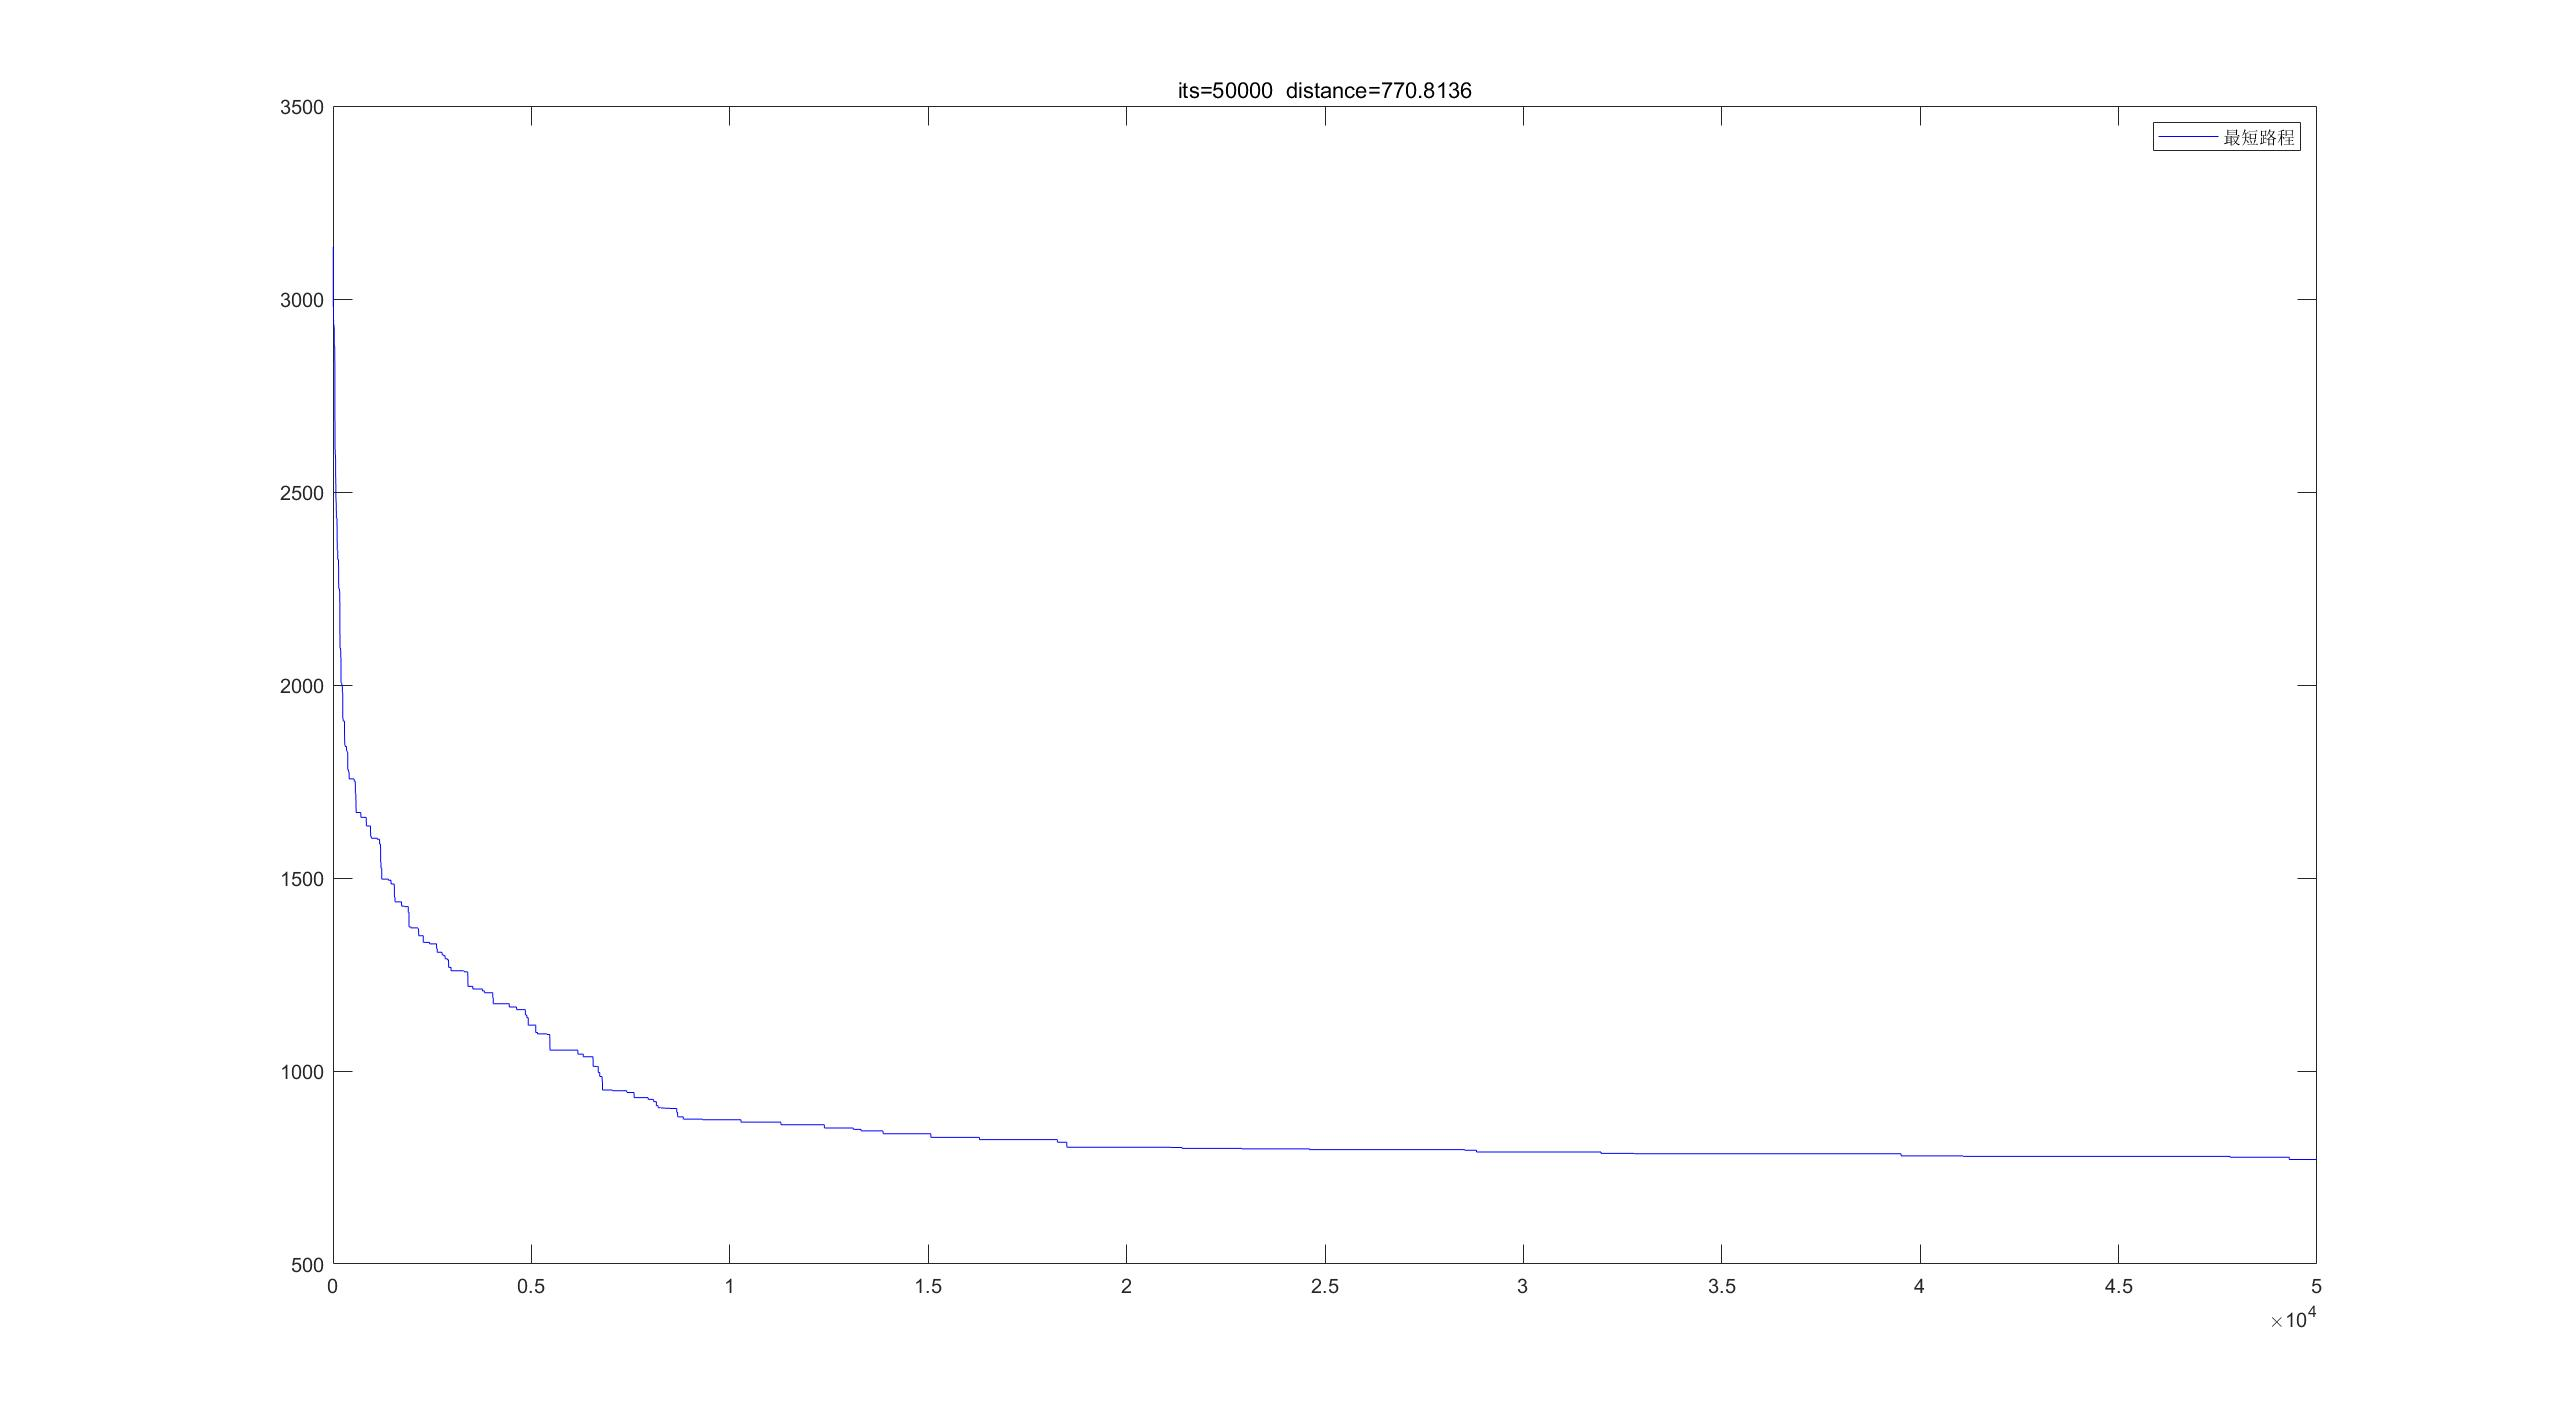
\includegraphics[scale=0.15]{figure1.jpg}
  \caption*{Picture of approach process}
\end{figure}
\newpage
\section*{Code}
All codes attached to homework could be found in \url{https://github.com/CyanCap/CI-code.git}.

\section*{Main function for part A:}
\begin{lstlisting}[language=matlab]
%probability for crossover and mutation. iterations and population size setting:
  xpro=0.9; insertpro=0.2;  swappro=0.3;  its=50; num=20;
  pop=initpop(dis,num);   %initialize population
  yopt=zeros(1,its);
  x=1:its;
  for i=1:its   %operate number of iterations times
    v1=totaldis(pop);   %calculate the total distance
    pop_1=selection(pop,v1);    %reproduction and selection
    pop_2=xover(pop_1,xpro);    %crossover with probability xpro
    pop_3=mutation_insert(pop_2,insertpro);   %insert mutation 
    pop_4=mutation_swap(pop_3,swappro);   %swap mutation
    v2=totaldis(pop_4);                       
    [indopt,disopt]=findopt(pop_4,v2);    %choose the optimal individuals
    if i<=1   %record the optimal path
      yopt(i)=disopt;
      path=indopt;
    else
      if yopt(i-1)>=disopt
          yopt(i)=disopt;
          path=indopt;
      else
          yopt(i)=yopt(i-1);
      end
    end
    drawnow;    %visualize the solution
    hold off
    plot(x,yopt,'b');
    title(['its=',num2str(i),'  distance=',num2str(yopt(i))]);
    legend('optimal distance');
    pop=pop_4;
    pop(end,:)=path;    %add optimal path to population
  end
\end{lstlisting}

\end{document}